% Title: Report LaTex File: Software Development
% Auther: DC Eksteen
% Student Number: 22623906
% Contact: 22623906@sun.ac.za
% Date: 2022/09/14
% Version: 2.0

\chapter{Software Development}
\label{ch:software}
The software that was developed for this project was written in object orientated Python 3, using Visual Studio Code code editor. The software was then deployed on a Raspberry Pi 3 B+ single-board computer. 

\newpage

\section{Structure}

A Raspberry Pi has been selected as micro-controller base for the trainer. This means that the application will run on Raspberry Pi OS (previously called Raspbian), which is a 32-bit Unix-like operating system based on the Debian Linux distribution that was specifically developed for the Raspberry Pi. Subsequently, the application software was developed to work with standard Linux system architecture to achieve the required functionality.

The subsystems that were leveraged for this project were the Bluez Library, dBus manager, 

\color{red}

The software for the project has been written to form a very modular structure with separate "handlers" being written/developed for different functions of the greater application. There are some exceptions where existing libraries and servers were used, but these are referenced in the relevant sections later in this chapter.\\
Figure \ref{fig:soft} below shows the modular structure that was implemented for the control of the Raspberry Pi 3B+ single-board computer

\begin{figure}[h!]
	\begin{center}
		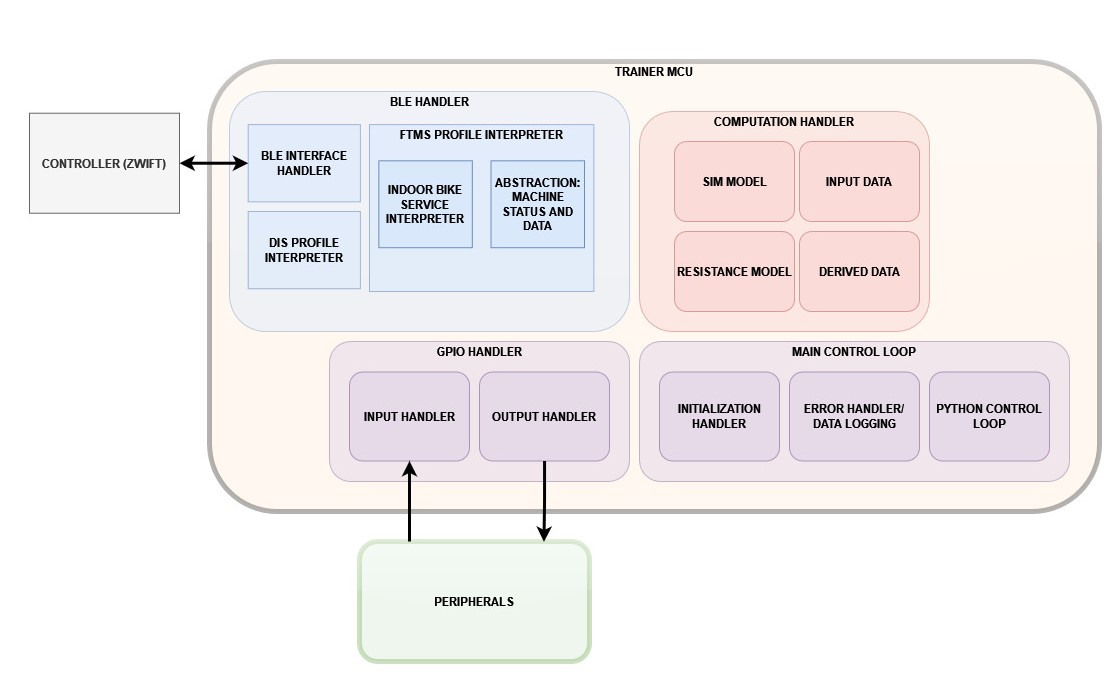
\includegraphics[width=1\textwidth]{Software.jpg}
		\caption{Overview of General Software Structure}
		\label{fig:soft}
	\end{center}
\end{figure}

\section{\ac{ble} Handler}
The \ac{ble} handler is responsible for all of the Bluetooth communication protocols, and has to strictly conform to the \ac{ble} specifications in order to ensure compatibility with common devices. The handler consists of a few different services that in tern manage some service or function within the greater protocol.\\
The \ac{ble} protocol was designed to be used with various layers of abstraction between the low level operations of the system. This results in the structure for the abstraction layers as seen in Figure \ref{fig:blez} below:

\begin{figure}[H]
	\begin{center}
		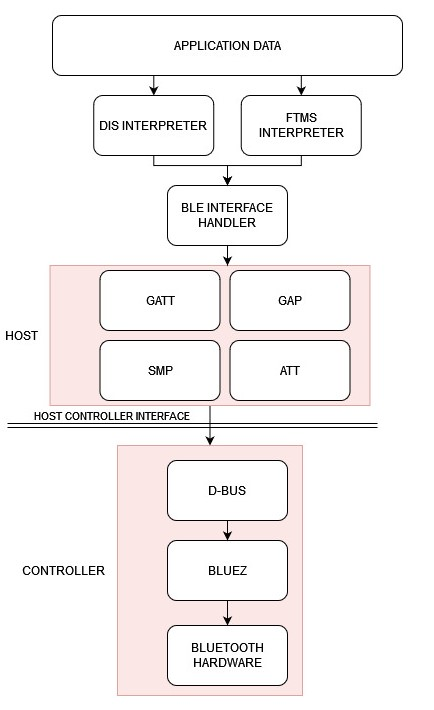
\includegraphics[width=0.5\textwidth]{BLEdiagram.jpg}
		\caption{\ac{ble} Protocol Stack}
		\label{fig:blez}
	\end{center}
\end{figure}

The abstraction all the way up to the host already exists and is implemented on the Raspberry Pi. The D-Bus is an \ac{ipc} method that allows for \ac{rpc} between the various processes. The role of the \ac{ble} Interface Handler is thus to handle communication between the main process and Bluez. Bluez is the official Linux Bluetooth protocol stack, and is what controls the Bluetooth operations of the system. \citep{Lee:2020}\\

The \ac{ftms} and \ac{dis} Interpreters receive and send various \ac{ble} commands, requests and replies between the \ac{ble} Interface Handler and the running application. It is here where messages are split up into their various components before being acted apron, and replies get created in the required format before being sent to the Bluez stack.

\newpage

\section{Sensor Data Measuring and Logging}

\newpage

\section{Power Calculations}

\begin{figure}[H]
	\begin{center}
		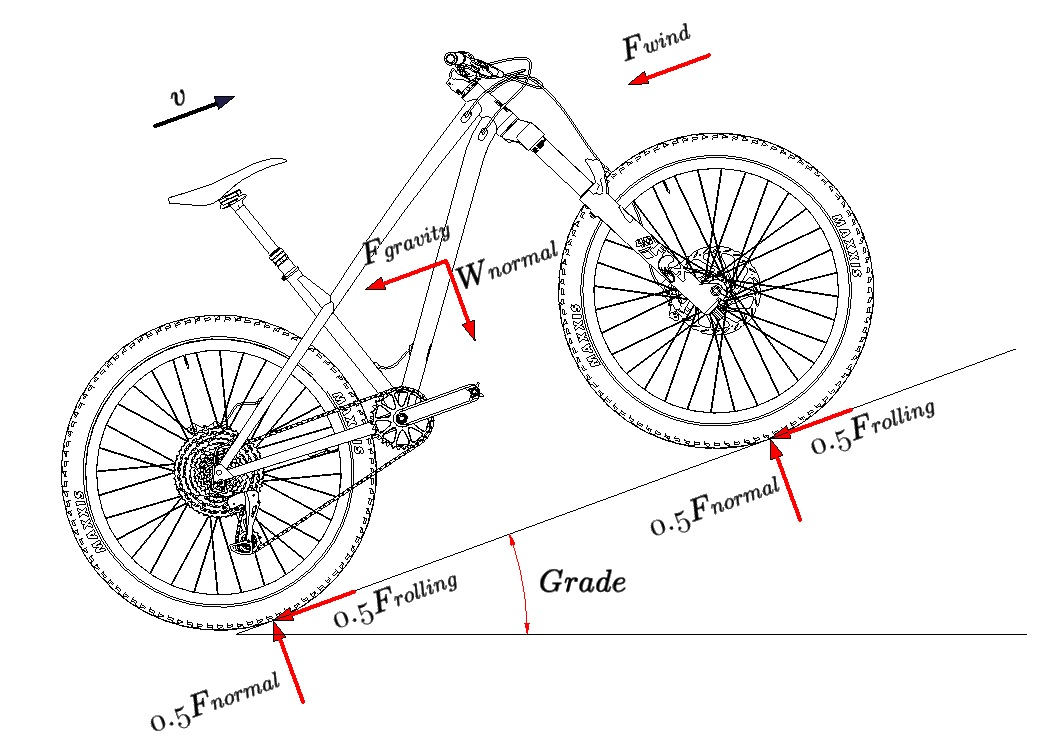
\includegraphics[width=0.8\textwidth]{SIM.jpg}
		\caption{Cycling Physics Illustration}
		\label{fig:sim}
	\end{center}
\end{figure}

\newpage

\section{Motor Control}

